\chapter{Initial system design}
In this chapter I'm introducing the initial design of the above mentioned system from both hardware and
software aspects. Since there are several unknown factors 
during this phase, the designs described in this chapter represent an initial or starting step. The actual
system design will be based on the experience gained during these simulations in several trial-and-error 
based iterations.



\section{Simulation}
Before actually building the system and experimenting on an expensive quadcopter in real world environment,
it is cheaper, safer and easier to do tests in a simulated environment. 

The PX4 Firmware repository\cite{PX4Repository} contains Gazebo simulation files to give developers a head 
start in the simulation of their product. Upon these quadcopter models the LIDAR sensors can be placed and 
moved around with ease, without the need of wiring or external infrastructure. This simulation is also 
suitable for Software in the loop (SITL) testing, meaning that the same software developed for the simulation
can be used on a real quadcopter. 

\subsection{Robot Operating System}
Robot Operating system (ROS) is a set of software libraries and tools that help developers to build robust 
general-purpose robot applications\cite{ROSWebsite}. ROS provides hardware abstraction of the underlying 
robot, generalizes the interfacing of these robots and allows simple usage using high level features.


The core component of ROS is a public-subscribe communication protocol similar to the well-known MQTT protocol
used on the field of IoT. The ROS system is comprised of a number of independent communicating parties called 
nodes. Each node can subscribe to multiple topics and receive a stream of messages published to these topics 
by other nodes. For example a temperature filter node might subscribe to a topic of "/temperature\_sensor" 
and publish the filtered temperature values to a topic called "/filtered\_temperature\_sensor". 
The benefit using this solution is that the nodes achieve communication exclusively via this protocol 
so each node can live independently from another.

Nodes in ROS do not need to be on the same system or even on the same architecture. Nodes can run on different 
computers or even on microcontrollers or smartphones.

\begin{figure}[!ht]
    \centering
    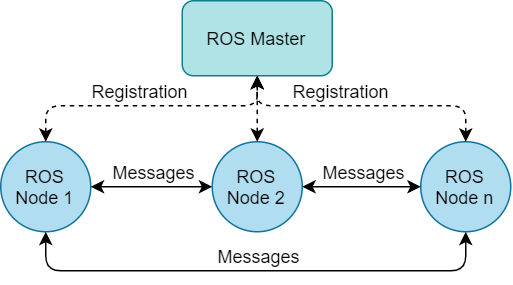
\includegraphics[width=100mm, keepaspectratio]{figures/ros_pubsub.png}
    \caption{ROS publish subscribe communication}
    \label{fig:ros_pubsub}
\end{figure}



\subsection{Gazebo}


\newpage
\section{Hardware plan}
\subsection{VL53L1X LIDAR}
\subsection{LIDAR placement}
\subsection{LIDAR data collection}
\subsubsection{Logging on SD Card}
\subsubsection{Wireless transceiver}
\subsubsection{Integrating messages into PX4 firmware}

\section{Software plan}